\documentclass[a4paper,12pt]{article}
\usepackage{graphicx}
\usepackage[a4paper,margin=1in]{geometry}
\usepackage{titlesec}
\usepackage{hyperref}
\usepackage{amsmath}    % For math environments and symbols
\usepackage{amssymb}    % For \mathbb and other math symbols
\usepackage{amsfonts}   % Additional math fonts
\usepackage{float}
\setlength{\abovecaptionskip}{-2pt}  
\setlength{\belowcaptionskip}{1pt}
\usepackage{subcaption}
\usepackage[numbers]{natbib}
\usepackage{makecell}
\usepackage{tikz}
\usetikzlibrary{arrows.meta, positioning}



% Title format
\titleformat{\section}{\large\bfseries}{\thesection}{1em}{}

% Title settings
\title{
    \includegraphics[scale=0.4]{Cam_logo_bw.png}\\
    \vspace{0.5cm}
    M2 Deep Learning - Coursework Assignment
}
\author{Raunaq Rai (rsr45@cam.ac.uk)\\
    Data Intensive Science, Department of Physics, University of Cambridge
}
\date{04 April, 2025 \\ \vspace{0.2cm} {\small Word Count: 2961}}

\begin{document}

\maketitle

\section*{Introduction}

Recent advances have demonstrated that Large Language Models (LLMs) can be effective not only in natural language tasks but also in domains such as time-series forecasting \citep{gruver2023language}. In this coursework, we explore the application of Low-Rank Adaptation (LoRA) \citep{hu2021lora} to the Qwen2.5-Instruct model \citep{qwen2.5}, a transformer-based LLM, for forecasting predator-prey population dynamics as described by the Lotka–Volterra equations \citep{takeuchi2006lotka}.

Utilising the preprocessing methodology in the LLMTIME framework \citep{gruver2023language}, we examine how Qwen2.5-Instruct can be repurposed for numerical prediction tasks. The objective is to fine-tune the model on a dataset of simulated predator-prey trajectories using LoRA, which allows for the adaptation of pretrained models without updating all weights.

This report describes the implementation of LLMTIME preprocessing, baseline evaluation of the untrained model, LoRA fine-tuning with hyperparameter sweeps, and analysis of forecasting performance under compute constraints.

\section{Compute Constraint}

This coursework requires efficient experimentation under a strict compute budget of $10^{17}$ floating point operations (FLOPs) across all reported experiments.

FLOP costs are calculated using simplified, hardware-agnostic assumptions. Table~\ref{tab:flops_primitives} provides the per-operation FLOP estimates:

\begin{table}[H]
  \centering

  \begin{tabular}{lc}
    \hline
    Operation & FLOPs \\
    \hline
    Addition / Subtraction / Negation (float or int) & 1 \\
    Multiplication / Division / Inverse (float or int) & 1 \\
    ReLU / Absolute Value & 1 \\
    Exponentiation / Logarithm & 10 \\
    Sine / Cosine / Square Root & 10 \\
    \hline
  \end{tabular}
  \vspace{0.2cm}
  \caption{FLOPs Accounting for Primitive Operations}
  \label{tab:flops_primitives}
\end{table}

\subsection*{FLOP Estimator Implementation}

To estimate the computational cost of each experiment, we implemented a FLOP estimator in Python (flops\_model.py and compute\_flops.py). This estimator models a forward pass through the Qwen2.5-0.5B architecture. These scripts were validated through a corresponding test set.

The estimator accounts for every trainable and non-trainable component of the model. For a given sequence length $n$, the estimator computes the total number of FLOPs for each of the following:

\begin{itemize}
  \item \textbf{Token Embeddings}: Retrieved via indexing and incur no arithmetic FLOPs.
  
  \item \textbf{Positional Embeddings}: Sinusoidal encodings are added to token embeddings, requiring $n \times d_{\text{model}}$ additions.

  \item \textbf{Multi-head Attention (per layer)}:
  \begin{itemize}
    \item Query, Key, and Value projections: Linear transformations to $d_{\text{head}}$ per head; includes multiplications and bias additions.
    \item Dot-product attention: Computation of $QK^\top$, scaling, softmax, and weighted sum with $V$.
    \item Softmax operation: Includes exponentiations, summations, and divisions.
    \item Output projection: Concatenation of heads followed by a linear transformation.
  \end{itemize}

  \item \textbf{Feedforward MLP with SwiGLU}: As described by \citet{shazeer2020glu}, this block consists of:
  \begin{itemize}
    \item Two parallel linear up-projections from the model dimension to the hidden dimension: one to produce the activation input, and one to produce the gating values.
    \item A SwiGLU activation function, which applies the SiLU nonlinearity to one stream and multiplies it elementwise with the other (gating).
    \item A final down-projection from the hidden dimension back to the model dimension.
  \end{itemize}  

  \item \textbf{RMSNorm Layers}: Following \citet{zhang2019root}, these involve:
  \begin{itemize}
    \item Elementwise squaring, summation, square root, division, and scaling by a learned parameter $\gamma$.
  \end{itemize}

  \item \textbf{LoRA Projections}: As proposed by \citet{hu2021lora}, LoRA introduces:
  \begin{itemize}
    \item Low-rank down-projection matrices and up-projection matrices are added to the frozen base weights.
    \item FLOPs from these include multiplications, additions, and a residual connection.
  \end{itemize}

  \item \textbf{Final Projection to Vocabulary Logits}:
  \begin{itemize}
    \item A linear layer projecting to the vocabulary space: $n \times d_{\text{model}} \times V$ multiplications and additions.
  \end{itemize}
\end{itemize}

The exact computation of FLOPs for backpropagation is non-trivial and implementation-specific. For the purposes of this coursework, we assume that the backward pass is approximately double the cost of the forward pass. This is a conservative estimate, as it does not account for optimisations such as gradient checkpointing or memory reuse.

Thus, the total training FLOPs are given by:
\begin{equation}
\text{FLOPs}_{\text{train}} \approx 3 \times \text{FLOPs}_{\text{forward}}
\end{equation}

\section{LLMTIME Preprocessing Implementation}


We implemented the LLMTIME preprocessing scheme \citep{gruver2023language} to convert multivariate time-series data into a format suitable for Qwen2.5-Instruct. This was done by creating a dedicated Python module (preprocessor.py) containing a class LLMTIMEPreprocessor, which formats and tokenizes time-series data into LLMTIME-style strings for model input.

The data used in this coursework consists of simulated trajectories from the Lotka–Volterra predator-prey system, a well-known model in population dynamics. Each time series contains 100 steps with two variables: prey population and predator population. The full dataset contains 1000 such trajectories stored in a single file.

\subsection*{Scaling and Formatting}

Each sample, consisting of a pair of sequences, can vary in magnitude both within and across samples. This can lead to inconsistent token lengths after formatting and limit the model’s ability to generalise.

To account for this, we compute a per-sample scaling factor $\alpha$ that normalises the numerical range before tokenization:
\begin{equation}
\alpha = \frac{1}{10} \cdot \max\left(\text{percentile}_{95}(\text{prey}),\ \text{percentile}_{95}(\text{predator})\right)
\end{equation}

We then divide each value in the prey and predator sequences by $\alpha$, ensuring that the majority of values fall within the range $[0, 10]$. This sample-specific scaling avoids the limitations of global normalisation and makes the model more robust to differences in scale across the dataset.

Finally, all scaled values are rounded to two decimal places. This rounding step reduces the number of unique numeric tokens, improving tokenization consistency and helping prevent overfitting to insignificant digit-level variation.


\subsection*{LLMTIME Encoding}

Following the LLMTIME convention, each timestep is represented as a pair of variables (prey, predator), separated by a comma. Consecutive timesteps are separated by a semicolon. While the original LLMTIME implementation by \citet{gruver2023language} removes decimal points to reduce sequence length, especially for GPT-style models that tokenize numbers into subword units, we keep the decimal point in our implementation for several important reasons:

\begin{itemize}
  \item Preserving the decimal enhances human interpretability and simplifies decoding during inference.
  \item The coursework specification explicitly recommends retaining the decimal point.
\end{itemize}

\subsection*{Tokenization}

Once formatted, the numeric string is passed through Qwen2.5’s tokenizer using Hugging Face’s AutoTokenizer interface \cite{huggingface}. Each digit and punctuation mark is tokenized into its own token. Two examples of this are shown below:

\paragraph{Example 1.}
\begin{itemize}
  \item \textbf{Original Input:}
  \begin{verbatim}
Prey:     [2.9, 3.2, 3.8, 4.5, 5.1]
Predator: [1.1, 0.9, 0.7, 0.6, 0.5]
  \end{verbatim}

  \vspace{-0.7cm}

  \item \textbf{Scale Factor $\alpha$:} 0.498


  \item \textbf{Formatted Sequence:}
  \begin{verbatim}
5.82,2.21;6.43,1.81;7.63,1.41;9.04,1.20;10.24,1.00
  \end{verbatim}

  \vspace{-0.7cm}

  \item \textbf{Tokenized Output (Qwen2.5 input IDs):}
  \begin{verbatim}
[20, 13, 23, 17, 11, 17, 13, 17, 16, 26, 21, 13, 19, 18, 11,
16, 13, 23, 16, 26, 22, 13, 21, 18, 11, 16, 13, 19, 16, 26,
24, 13, 15, 19, 11, 16, 13, 17, 15, 26, 16, 15, 13, 17, 19,
11, 16, 13, 15, 15]
  \end{verbatim}
\end{itemize}

\vspace{-1cm}

\paragraph{Example 2.}
\begin{itemize}
  \item \textbf{Original Input:}
  \begin{verbatim}
Prey:     [1.5, 1.8, 2.1, 2.4, 2.7]
Predator: [2.8, 2.5, 2.2, 1.9, 1.6]
  \end{verbatim}

  \vspace{-0.7cm}

  \item \textbf{Scale Factor $\alpha$:} 0.274

  \item \textbf{Formatted Sequence:}
  \begin{verbatim}
5.47,10.22;6.57,9.12;7.66,8.03;8.76,6.93;9.85,5.84
  \end{verbatim}

  \vspace{-0.7cm}

  \item \textbf{Tokenized Output (Qwen2.5 input IDs):}
  \begin{verbatim}
[20, 13, 19, 22, 11, 16, 15, 13, 17, 17, 26, 21, 13, 20, 22,
11, 24, 13, 16, 17, 26, 22, 13, 21, 21, 11, 23, 13, 15, 18,
26, 23, 13, 22, 21, 11, 21, 13, 24, 18, 26, 24, 13, 23, 20,
11, 20, 13, 23, 19]
  \end{verbatim}
\end{itemize}

\begin{figure}[H]
  \centering

  \begin{subfigure}[H]{0.8\textwidth}
      \centering
      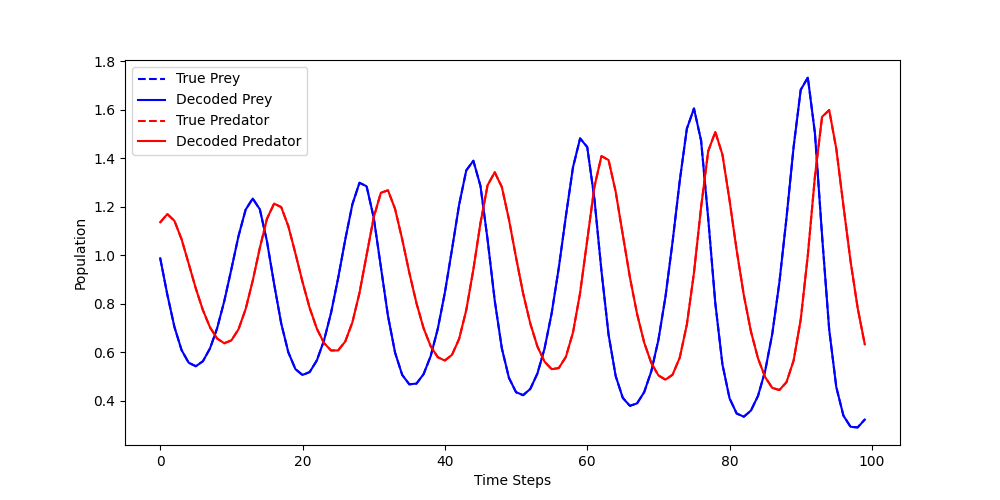
\includegraphics[width=\textwidth]{true_vs_decoded.png}
      \caption{Decoded output vs.\ ground truth for the 972\textsuperscript{nd} Lotka-Volterra trajectory in the test set. This sequence was passed through the LLMTIME preprocessing pipeline, the resulting output was decoded and rescaled using the same scale factor $\alpha$ applied during encoding.}
      \label{fig:true_vs_decoded}
  \end{subfigure}

  \vspace{0.5cm}

  \begin{subfigure}[H]{0.8\textwidth}
      \centering
      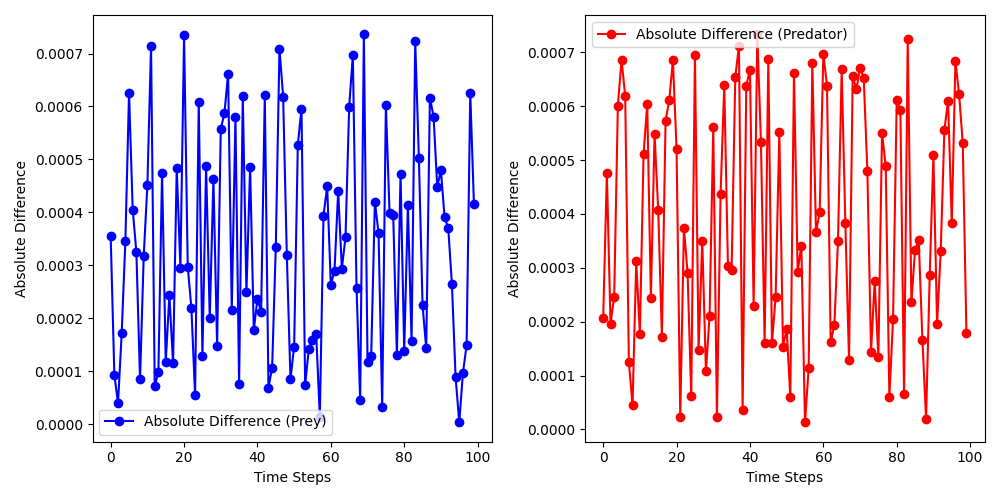
\includegraphics[width=\textwidth]{absolute_differences.png}
      \caption{Absolute differences between true and decoded prey (left) and predator (right) values for the 972\textsuperscript{nd} test sequence.  The close alignment between original and decoded values confirms that the preprocessing, tokenization, and decoding pipeline is working as intended.}
      \label{fig:absolute_differences}
  \end{subfigure}
  \vspace{0.5cm}
  \caption{ Encoding - Decoding check for Sample 972.}
  \label{fig:decoding_pipeline_evaluation}
\end{figure}

  
\section{Baseline Evaluation}

We assessed the forecasting ability of the untrained Qwen2.5-0.5B-Instruct model \cite{qwen2.5} using Sample ID 972. The first 50 timesteps were provided as input in LLMTIME format, and the model was tasked with generating the remaining 50 steps.

Using the Hugging Face generate() API \cite{huggingface}, the model predicted one token at a time, with each new token requiring a full forward pass.

\subsection*{Forecasting Performance}

We evaluate the model's forecasting accuracy on Sample ID 972 by comparing the decoded and rescaled predictions to the true population values using standard regression metrics. The results are summarised below:

\begin{itemize}
  \item \textbf{Prey Population}
  \begin{itemize}
    \item Mean Squared Error (MSE): 0.3812
    \item Mean Absolute Error (MAE): 0.3597
    \item Coefficient of Determination ($R^2$ Score): -1.7590
  \end{itemize}

  \item \textbf{Predator Population}
  \begin{itemize}
    \item Mean Squared Error (MSE): 0.1324
    \item Mean Absolute Error (MAE): 0.1904
    \item Coefficient of Determination ($R^2$ Score): -0.4884
  \end{itemize}
\end{itemize}

The negative $R^2$ scores for both prey and predator indicate that the model performs worse than a simple mean-based baseline.

  Due to the autoregressive nature of language models and the sampling-based decoding used during generation, repeated runs on the same input often give different output sequences. This non-determinism, unless explicitly controlled with fixed seeds or deterministic decoding settings, contributes to the variability in forecasting performance across trials.
  
  \begin{figure}[h]
      \centering
      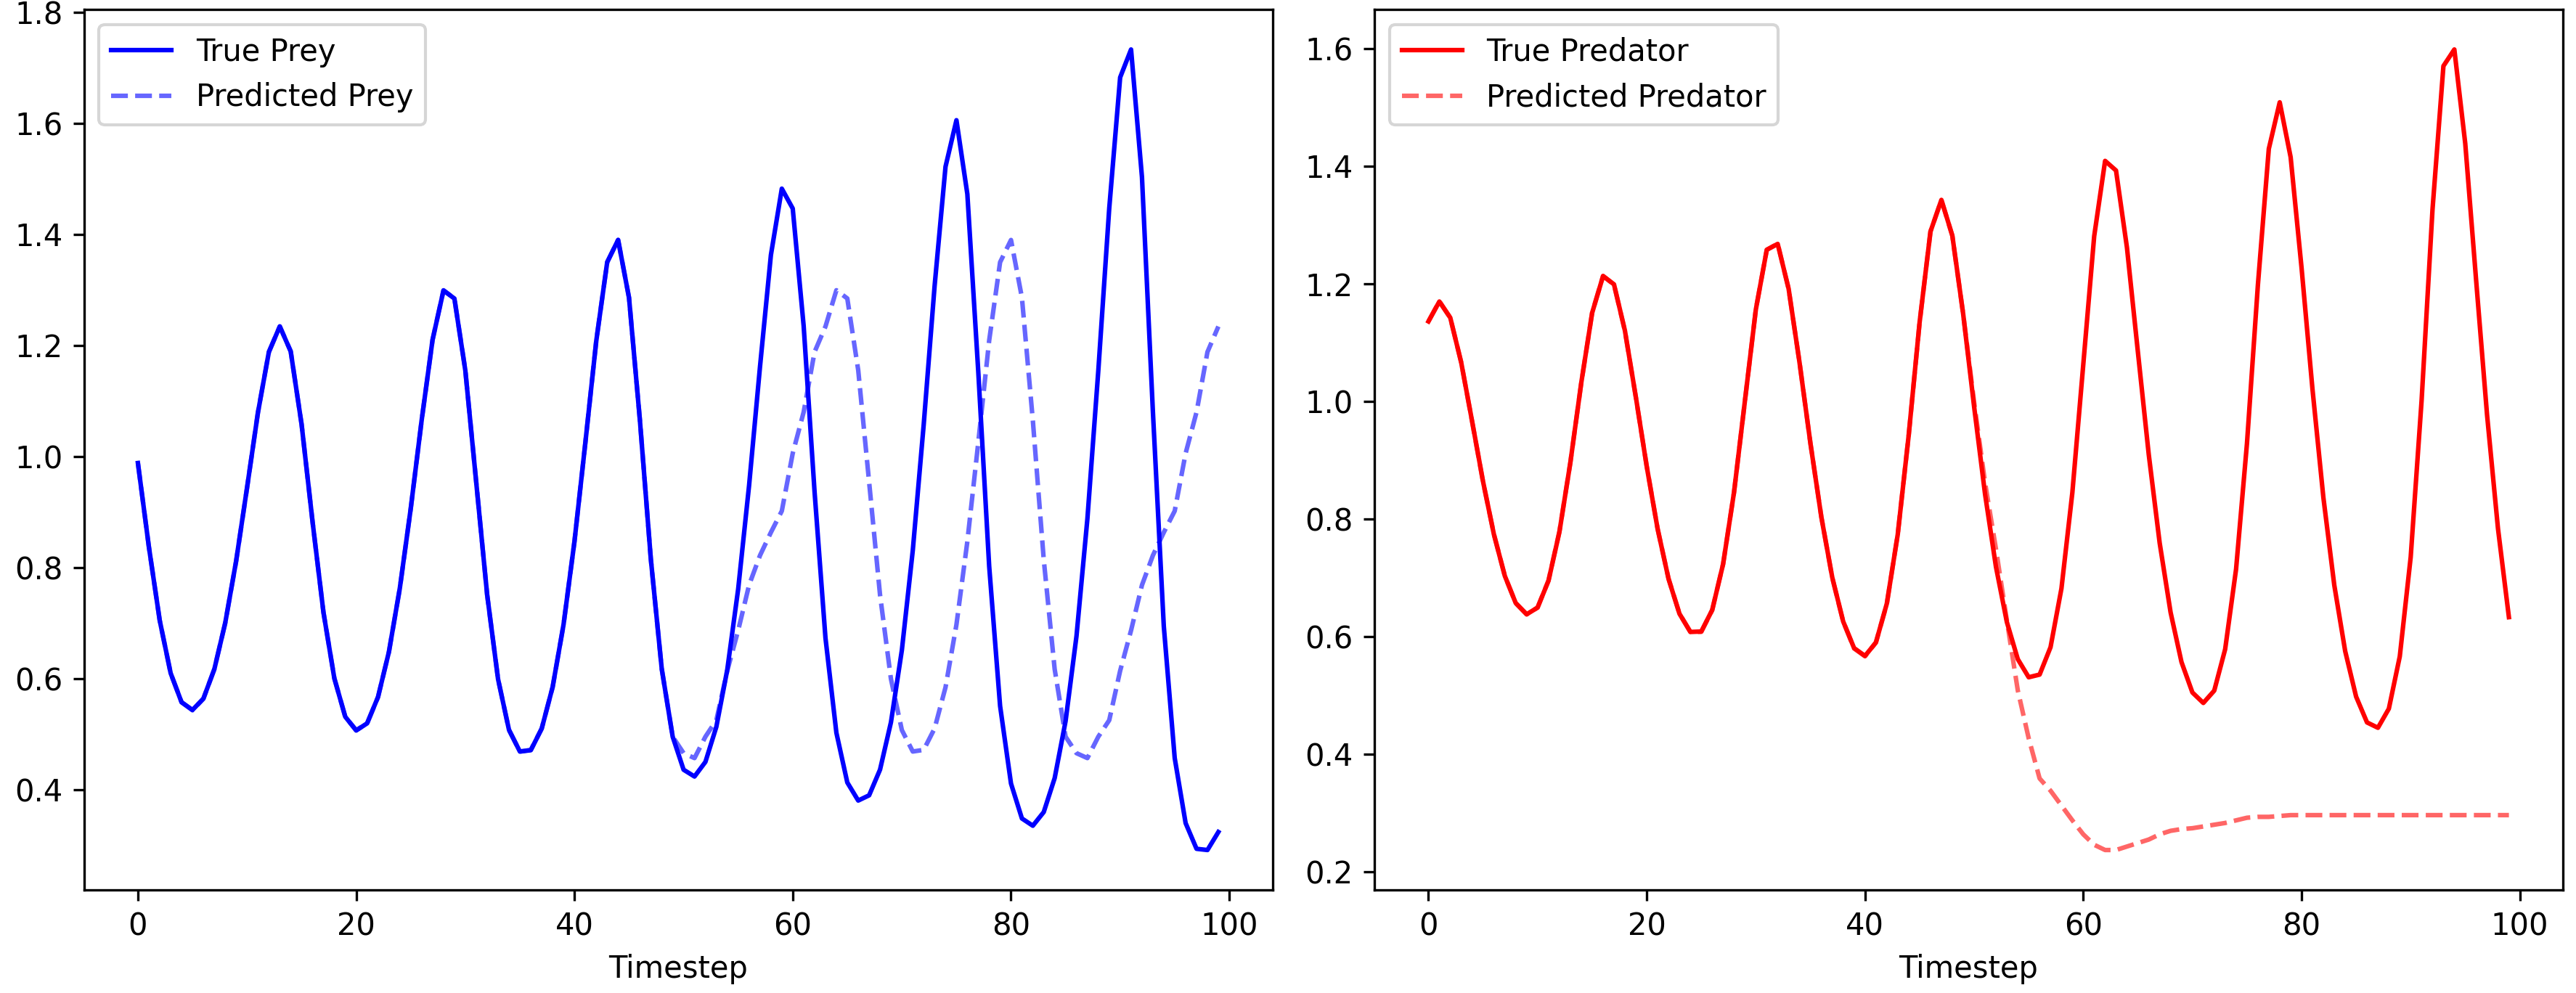
\includegraphics[width=0.9\textwidth]{sample972_untrained.png}
      \caption{Forecasting output of the untrained Qwen2.5-Instruct model on Sample ID 972. The model is prompted with the first 50 timesteps and generates the next 50.}
      \label{fig:sample972_untrained}
  \end{figure}
  

  \section{FLOP Model}

To calculate the total FLOPs used by the Qwen2.5-0.5B-Instruct model, we mapped every major component in the forward pass to arithmetic operations and computed their FLOP costs using Table~\ref{tab:flops_primitives}. For inference, we assume reuse of Key/Value caches, meaning dot-product attention scores are only computed for new tokens, not the full input sequence.

\subsection*{Token and Positional Embeddings}
\begin{itemize}
  \item \textbf{Token Embeddings:} Retrieved via table lookup — \textbf{0 FLOPs}.
  \item \textbf{Positional Embedding Addition:} $n \times d_{\text{model}}$ additions.
\end{itemize}

\subsection*{RMSNorm (applied before attention, after attention, and before MLP)}

The Root Mean Square Layer Normalisation (RMSNorm) \citep{zhang2019root} normalises each input token $x \in \mathbb{R}^d$ using the root mean square of its elements, without subtracting the mean. The operation is defined as:
\begin{equation}
\text{RMSNorm}(x) = \frac{x}{\sqrt{\frac{1}{d} \sum_{i=1}^{d} x_i^2 + \epsilon}} \cdot \gamma
\end{equation}
where $\gamma \in \mathbb{R}^d$ is a learned scaling parameter and $\epsilon$ is a small constant for numerical stability.

For a batch of $n$ tokens (each of dimension $d$), the FLOPs are as follows:
\begin{itemize}
  \item Square each element: $n \times d$ multiplications.
  \item Sum across dimensions: $n \times (d - 1)$ additions.
  \item Compute the square root of the mean: $n$ square root operations.
  \item Divide each element by the norm: $n \times d$ divisions.
  \item Scale with learned weight $\gamma$: $n \times d$ multiplications.
\end{itemize}

\textbf{Total:} $2nd$ multiplications, $n(d - 1)$ additions, $nd$ divisions, $n$ square roots.


\subsection*{Multi-Head Attention (per layer)}
Let $h$ be the number of heads and $d_h = d / h$ which refers to the dimensionality fo each attention head.
\begin{itemize}
  \item \textbf{Q/K/V Projections:} $3 \times n \times d \times d_h$ multiplications and $3 \times n \times (d - 1) \times d_h$ additions.
  \item \textbf{Attention Scores:} $n \times n \times d_h$ multiplications and $n \times n \times (d_h - 1)$ additions.
  \item \textbf{Softmax:} For $n^2$ elements:
    \begin{itemize}
      \item Exponentiation: $n^2$
      \item Summation: $n \times (n - 1)$ additions
      \item Normalisation: $n^2$ divisions
    \end{itemize}
  \item \textbf{Softmax-Value Multiplication:} $n \times n \times d_h$ multiplications and $n \times d_h \times (n - 1)$ additions.
  \item \textbf{Concatenation:} Memory operation — \textbf{0 FLOPs}.
  \item \textbf{Final Output Projection:} $n \times d \times d$ multiplications and $n \times (d - 1) \times d$ additions.
\end{itemize}

\subsection*{MLP Block with SwiGLU (per layer)}

Let $d$ be the model embedding dimension, $d_{\text{ff}}$ the hidden (feedforward) dimension, and $n$ the number of tokens in the sequence. The MLP block consists of two parallel up-projections (one gated) and a down-projection, followed by a SwiGLU activation \citep{shazeer2020glu}.

\begin{itemize}
  \item \textbf{Up-Projections and Gating:} Two parallel linear layers (one for gate, one for activation) each compute:
  \[
  \text{Multiplications: } n \times d \times d_{\text{ff}}, \quad
  \text{Additions: } n \times (d - 1) \times d_{\text{ff}}
  \]
  Multiplied by 2 for both paths:
  \[
  \Rightarrow 2 \times n \times d \times d_{\text{ff}} \text{ multiplications, and } 2 \times n \times (d - 1) \times d_{\text{ff}} \text{ additions.}
  \]

  \item \textbf{SwiGLU Activation:} The gated activation combines SiLU and elementwise multiplication:
  \begin{itemize}
    \item Each unit requires: 1 exponentiation, 1 division, 2 multiplications, and 1 addition.
    \item Total per token: $n \times d_{\text{ff}}$ of each (add, div, exp) and $2 \times n \times d_{\text{ff}}$ multiplications.
  \end{itemize}

  \item \textbf{Down-Projection:} A single linear layer reduces dimensionality:
  \[
  \text{Multiplications: } n \times d_{\text{ff}} \times d, \quad
  \text{Additions: } n \times (d_{\text{ff}} - 1) \times d
  \]
\end{itemize}


\subsection*{Final Projection to Vocabulary Logits}

At the final stage of the model, the hidden representation for each token is projected into the vocabulary space to compute logits over all possible output tokens. This is done via a single linear transformation with weight matrix $W \in \mathbb{R}^{V \times d}$, where $V$ is the vocabulary size and $d$ is the model's hidden dimension.

\begin{itemize}
  \item \textbf{Multiplications:} For each of the $n$ tokens in the sequence, we compute a dot product between the hidden vector and each of the $V$ vocabulary embeddings — resulting in $n \times d \times V$ multiplications.
  \item \textbf{Additions:} Each of those dot products involves $d-1$ additions, giving a total of $n \times (d - 1) \times V$ additions.
\end{itemize}

\subsection*{LoRA Projections}

LoRA replaces a standard linear layer $W \in \mathbb{R}^{d \times d}$ with a low-rank approximation consisting of two smaller matrices:
\begin{itemize}
  \item A \textbf{down-projection} matrix $A \in \mathbb{R}^{r \times d}$ (reducing dimensionality),
  \item An \textbf{up-projection} matrix $B \in \mathbb{R}^{d \times r}$ (projecting back to the original space).
\end{itemize}

Let:
\begin{itemize}
  \item $n$ be the number of tokens in the input sequence,
  \item $d$ be the model's hidden dimension,
  \item $r$ be the LoRA rank.
\end{itemize}

\begin{itemize}
  \item \textbf{Down-Projection ($A x$):} Projects from $\mathbb{R}^{d}$ to $\mathbb{R}^{r}$:
  \begin{itemize}
    \item Multiplications: $n \times d \times r$
    \item Additions: $n \times (d - 1) \times r$
  \end{itemize}

  \item \textbf{Up-Projection ($B (A x)$):} Projects from $\mathbb{R}^{r}$ back to $\mathbb{R}^{d}$:
  \begin{itemize}
    \item Multiplications: $n \times r \times d$
    \item Additions: $n \times (r - 1) \times d$
  \end{itemize}

  \item \textbf{Scaling and Residual Addition:} The result is scaled (typically by $\alpha / r$) and added to the original output:
  \begin{itemize}
    \item Multiplications: $n \times d$
    \item Additions: $n \times d$
  \end{itemize}
\end{itemize}

\textbf{Total FLOPs for one LoRA adapter:}
\begin{itemize}
  \item \textbf{Multiplications:} $2 \times n \times d \times r + n \times d$
  \item \textbf{Additions:} $2 \times n \times d \times r + n \times d$ (approximately)
\end{itemize}
This total assumes that both the down and up projections are active and used once per token per transformer block.

The total FLOPs are computed as:
\begin{equation}
\text{Total FLOPs} = \sum_{i=1}^{n} \left( a_i + m_i + d_i + 10e_i + 10s_i \right)
\end{equation}
where $a_i$, $m_i$, $d_i$, $e_i$, and $s_i$ represent the counts of additions, multiplications, divisions, exponentiations, and square roots respectively.

\section{LoRA Adaptation and Fine-Tuning Procedure}

Low-Rank Adaptation enablea parameter-efficient fine-tuning of the Qwen2.5-0.5B-Instruct model. It is applied to the query (Q) and value (V) projection layers in each transformer block. Specifically, we wrapped each of these layers with a custom LoRALinear module that augments the frozen base projection with a trainable low-rank update.

For each modified projection layer, we introduced two trainable matrices:
\begin{itemize}
    \item A down-projection matrix $A \in \mathbb{R}^{r \times d}$
    \item An up-projection matrix $B \in \mathbb{R}^{d \times r}$
\end{itemize}

The output of a LoRA-adapted linear layer becomes:

\begin{equation}
\text{output} = W x + \frac{\alpha}{r} B A x
\end{equation}
where $W$ is the original frozen weight matrix and $\alpha$ is a scaling factor (typically set equal to $r$) \citep{hu2021lora}.

We fine-tuned only the LoRA parameters ($A$, $B$) while keeping the base model parameters frozen. The adapted layers were implemented by replacing q\_proj and v\_proj in each transformer block.

\usetikzlibrary{arrows.meta, positioning, shapes.geometric}
\begin{figure}[h]
\centering
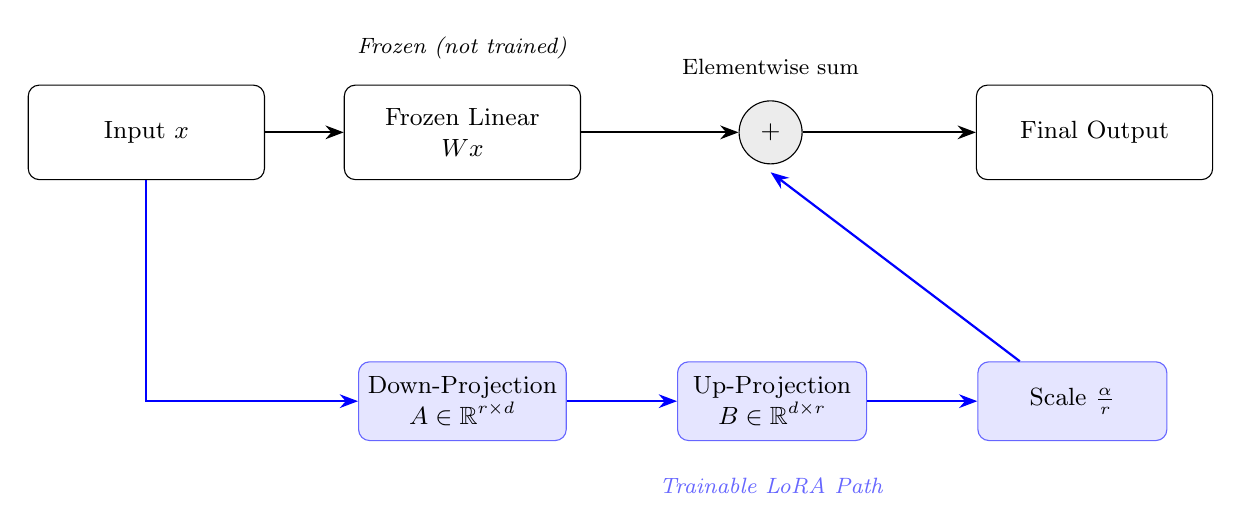
\begin{tikzpicture}[
    node distance=1.6cm and 1.4cm,
    every node/.style={font=\small},
    box/.style={rectangle, draw=black, rounded corners, minimum width=3cm, minimum height=1.2cm, align=center},
    lora/.style={rectangle, draw=blue!60, rounded corners, minimum width=2.4cm, minimum height=1cm, align=center, fill=blue!10},
    sum/.style={circle, draw=black, fill=gray!15, minimum size=0.8cm, inner sep=0pt},
    arrow/.style={-Stealth, thick},
    larrow/.style={-Stealth, thick, blue}
]

\node[box] (input) {Input $x$};
\node[box, right=1cm of input] (frozen) {Frozen Linear \\ $Wx$};
\node[sum, right=2.0cm of frozen] (add) {$+$};
\node[box, right=2.2cm of add] (output) {Final Output};

\node[lora, below=2.3cm of frozen] (A) {Down-Projection \\ $A \in \mathbb{R}^{r \times d}$};
\node[lora, right=of A] (B) {Up-Projection \\ $B \in \mathbb{R}^{d \times r}$};
\node[lora, right=of B] (scale) {Scale $\frac{\alpha}{r}$};

\draw[arrow] (input) -- (frozen);
\draw[arrow] (frozen) -- (add);
\draw[arrow] (add) -- (output);

\draw[larrow] (input) |- (A);
\draw[larrow] (A) -- (B);
\draw[larrow] (B) -- (scale);
\draw[larrow] (scale) -- ([yshift=-0.1cm]add.south);

\node[above=0.2cm of frozen] {\footnotesize \textit{Frozen (not trained)}};
\node[below=0.35cm of B] {\footnotesize \textcolor{blue!60}{\textit{Trainable LoRA Path}}};
\node[above=0.2cm of add] {\footnotesize Elementwise sum};

\end{tikzpicture}
\caption{LoRA adaptation of a linear layer. Only the blue LoRA path is trained; the original weights ($W$) are frozen. The output of the LoRA branch is scaled before being added to the frozen path.}
\label{fig:lora-flow-clear}
\end{figure}

Training was performed for 600 steps using default hyperparameters:
\begin{itemize}
    \item \texttt{lora\_rank} = 4
    \item \texttt{learning\_rate} = 1e-5
    \item \texttt{batch\_size} = 4
    \item \texttt{context\_length} = 512
\end{itemize}

We compared the trained model against an untrained baseline (LoRA-enabled but with zero optimisation steps). Both models were evaluated on a held-out validation set of 200 trajectories.
Evaluation was performed using cross-entropy loss, which measures how well the model's predicted probability distribution aligns with the true token distribution:

\begin{equation}
  \mathcal{L}_{\text{CE}} = - \frac{1}{T} \sum_{t=1}^{T} \log p_\theta(y_t \mid y_{<t}) = - \frac{1}{T} \sum_{t=1}^{T} \log p_\theta(y_t \mid y_1, y_2, \dots, y_{t-1})
\end{equation}

Here, $T$ denotes the total number of tokens in the sequence. The term $y_t$ represents the ground truth token at position $t$, while $y_{<t}$ refers to the sequence of all previous tokens from position 1 up to $t-1$. The model, parameterised by $\theta$, estimates the conditional probability $p_\theta(y_t \mid y_{<t})$, which is the probability it assigns to the correct next token given the preceding context.


\subsection*{Results}

\begin{itemize}
    \item \textbf{Untrained model (LoRA only, 0 steps):} Validation loss = \textbf{1.1926}
    \item \textbf{LoRA-trained model (600 steps):} Validation loss = \textbf{0.9651}
\end{itemize}

The performance improvement demonstrates that even a modest number of training steps is sufficient to adapt the model to the domain of Lotka–Volterra trajectories.

\section{LoRA Hyperparameter Search}

To understand how key hyperparameters affect forecasting performance, we carried out a targeted grid search over:
\begin{itemize}
    \item \textbf{LoRA Rank} $\in \{2, 4, 8\}$
    \item \textbf{Learning Rate} $\in \{10^{-5}, 5 \times 10^{-5}, 10^{-4}\}$
\end{itemize}

Increasing the LoRA rank introduces more trainable parameters per adapted layer, improving flexibility but increasing FLOP usage. The learning rate controls the speed of adaptation: values that are too high may destabilise training, while those too low may cause underfitting or slow convergence.

Each configuration was trained for 600 optimiser steps and evaluated on a held-out validation set — cross-entropy loss was used as the primary metric to quantify forecasting accuracy in token space. Due to FLOP constraints and clear trends in performance, not all combinations were run: validation loss consistently decreased as we moved to a higher LoRA rank and to a higher learning rate. These trends allowed us to avoid redundant runs while still identifying the most promising setup.

\vspace{0.2cm}

\begin{table}[H]
  \centering
  \begin{tabular}{|c|c|c|c|}
      \hline
      \textbf{LoRA Rank} & \textbf{LR = $10^{-4}$} & \textbf{LR = $5 \times 10^{-5}$} & \textbf{LR = $10^{-5}$} \\
      \hline
      2 & 
      \makecell{0 steps \\ 0.0000\% \\ n/a} & 
      \makecell{600 steps \\ 4.2212\% \\ 0.8099} & 
      \makecell{0 steps \\ 0.0000\% \\ n/a} \\
      \hline
      4 & 
      \makecell{600 steps \\ 4.22252\% \\ 0.6515} & 
      \makecell{600 steps \\ 4.22252\% \\ 0.7351} & 
      \makecell{600 steps \\ 4.22252\% \\ 0.9651} \\
      \hline
      8 & 
      \makecell{600 steps \\ 4.22516\% \\ 0.6162} & 
      \makecell{600 steps \\ 4.22516\% \\ 0.6744} & 
      \makecell{0 steps \\ 0.0000\% \\ n/a} \\
      \hline
  \end{tabular}
  \vspace{0.2cm}
  \caption{LoRA Hyperparameter Search Results. Each cell contains: training steps (top), percentage of FLOPs used (middle), and validation loss (bottom). Results for LoRA rank=4 and LR=1e-5 were reused from the previous section}
  \label{tab:lora_grid_search}
\end{table}

As shown in Table~\ref{tab:lora_grid_search}, the best-performing configuration used LoRA rank 8 and a learning rate of $10^{-4}$, achieving a validation loss of 0.6147.

\subsection*{Effect of Context Length on Forecasting Performance}

We next explored how the model’s performance is influenced by context length—the number of input tokens the model sees at once. Using the same LoRA rank (8) and learning rate ($10^{-4}$), we trained models using context lengths of \{128, 512 (already done), 768\}:

\begin{table}[H]
  \centering
  \begin{tabular}{|c|c|c|c|}
    \hline
    \textbf{Context Length} & \textbf{Validation Loss} & \textbf{Optimiser Steps} & \textbf{FLOPs Used (\%)} \\
    \hline
    128 & 0.7229 & 600 & 1.02421 \\
    512 & 0.6147 & 600 & \textit{(from previous section)} 4.22516 \\
    768 & 0.4207 & 600 & 6.46607 \\
    \hline
  \end{tabular}
  \vspace{0.2cm}
  \caption{Effect of context length on validation loss using LoRA rank 8 and learning rate $10^{-4}$.}
  \label{tab:context_length_results}
\end{table}

As expected, validation loss improves with increasing context length: longer contexts provide the model with more of the input sequence, enabling it to learn temporal patterns.

However, this benefit comes at a computational cost. Moving from 128 to 768 tokens increases the proportion of total FLOPs used from approximately 1\% to over 6\%, with the same number of training steps.

\section{Final Model Training and Evaluation}

We selected the following hyperparameters for our final model configuration:
\begin{itemize}
    \item \textbf{LoRA Rank:} 8
    \item \textbf{Learning Rate:} $10^{-4}$
    \item \textbf{Context Length:} 768
\end{itemize}

We trained the model for 5,000 steps using this setup, which was approximately 51.90\% of the total FLOP budget. Evaluation on a held-out validation set yielded a final loss of 0.2981 and a perplexity of 1.35.

\begin{figure}[H]
    \centering
    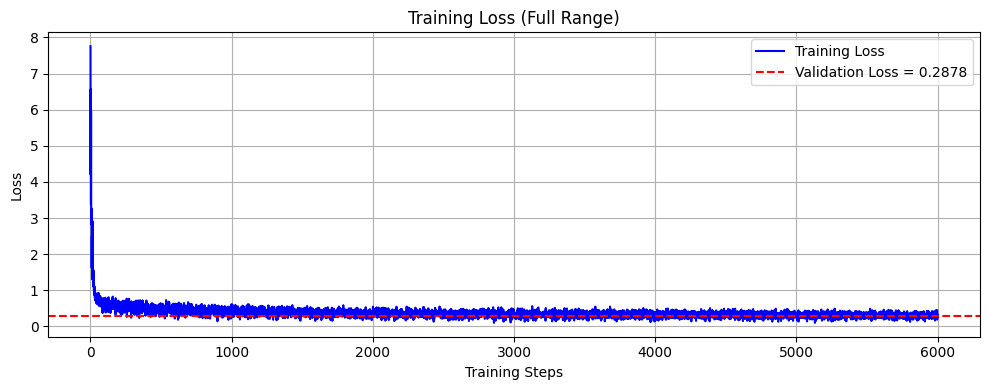
\includegraphics[width=0.85\linewidth]{training_loss.png}
    \caption{Training loss curve for the full 5,000-step run. The dashed red line indicates final validation loss.}
    \label{fig:training_loss}
\end{figure}

\begin{figure}[H]
    \centering
    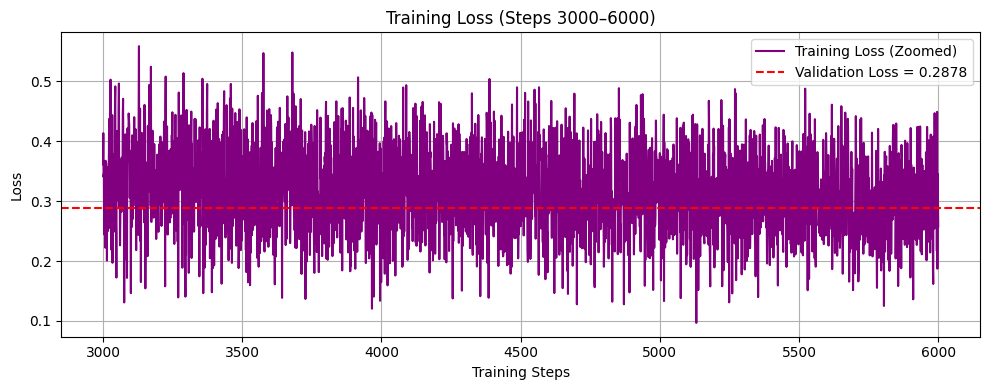
\includegraphics[width=0.85\linewidth]{zoomed_training_loss.png}
    \caption{Training loss over the last 2,500 steps.}
    \label{fig:zoomed_training_loss}
\end{figure}

The validation loss is comparable to the training loss throughout, suggesting that the model generalises well to unseen data and is not overfitting.

\subsection*{Evaluation}

To assess forecasting performance, we used the trained model to generate and visualise predictions on Sample ID 972. As shown in Figure~\ref{fig:sample_prediction}, the model closely tracks the ground-truth oscillatory behaviour of both prey and predator populations.
We also generate predictions for samples 990 - 999 in the test set to compute key evaluation metrics as shown in table \ref{tab:avg_metrics_990_999}.

\begin{figure}[H]
    \centering
    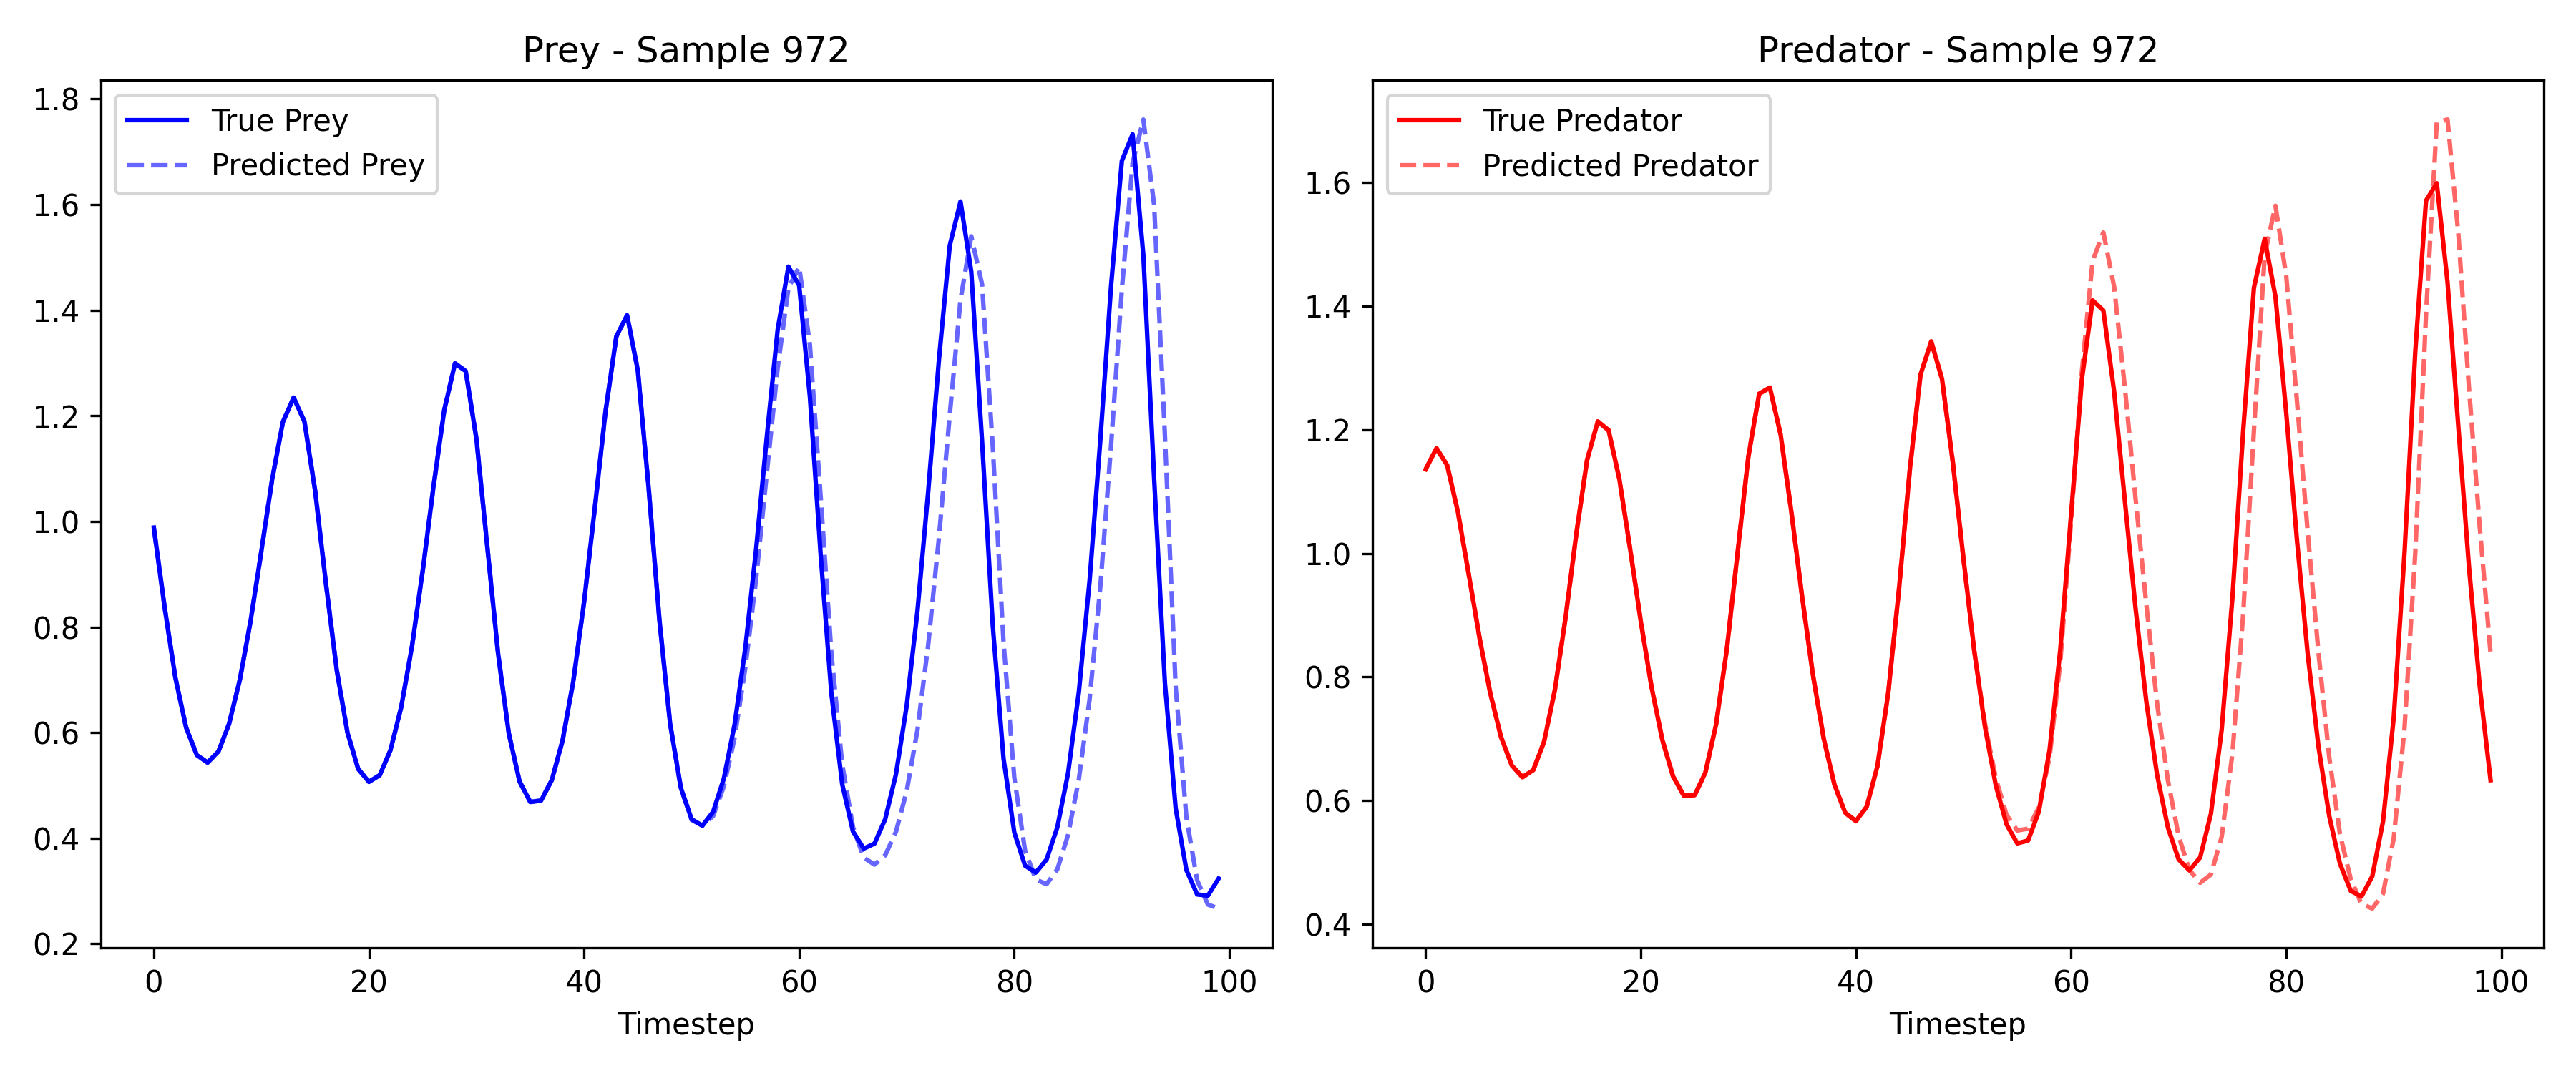
\includegraphics[width=0.95\linewidth]{sample972_trained.png}
    \caption{Forecasting results on Sample 972.}
    \label{fig:sample_prediction}
\end{figure}

\begin{table}[H]
    \centering

    \begin{tabular}{|c|c|c|c|}
        \hline
        \textbf{Species} & \textbf{MSE} & \textbf{MAE} & \textbf{R$^2$} \\
        \hline
        Prey & 0.0170 & 0.0671 & 0.8772 \\
        Predator & 0.0125 & 0.0608 & 0.8600 \\
        \hline
    \end{tabular}
    \vspace{0.2cm}
    \caption{Evaluation metrics for Sample 972}
    \label{tab:metrics_sample972}
\end{table}

\begin{table}[H]
  \centering
  \begin{tabular}{|c|c|c|c|}
      \hline
      \textbf{Target} & \textbf{MSE} & \textbf{MAE} & \textbf{R$^2$} \\
      \hline
      Prey & 0.1178 & 0.1483 & 0.8155 \\
      Predator & 0.0250 & 0.0687 & 0.7004 \\
      \hline
  \end{tabular}
  \vspace{0.2cm}
  \caption{Average evaluation metrics for samples 990–999.}
  \label{tab:avg_metrics_990_999}
  \end{table}

  Our experiments demonstrate that LLMs can be fine-tuned for time-series forecasting with tight FLOP constraints.
  
  The final model (LoRA rank 8, LR=$10^{-4}$, context length 768) achieved improved prediction accuracy for sample 972 representing a great improvement over the untrained model, which exhibited negative $R^2$ values and unstable forecasts.
  
  \section{Conclusion}

  This project demonstrates that large language models can be effectively repurposed for time-series forecasting under compute constraints when enhanced with parameter-efficient techniques like Low-Rank Adaptation. By integrating the LLMTIME preprocessing framework, adopting a FLOP-aware design, and performing systematic hyperparameter tuning, we successfully adapted Qwen2.5-Instruct to model predator-prey dynamics as described by the Lotka–Volterra equations. Our experimental results indicate that increasing the LoRA rank incurs only a marginal increase in FLOP usage compared to full fine-tuning—a cost that is outweighed by the improvements in forecasting accuracy. Notably, our final configuration—with a LoRA rank of 8, a learning rate of $10^{-4}$, and a context length of 768—achieved promising predictive performance while operating within the $10^{17}$ FLOP budget.
  
  Our work also showed several considerations for future research. The inherent non-determinism in autoregressive decoding leads to variability in the generated outputs, highlighting the importance of incorporating techniques to control or account for randomness during evaluation. Our hyperparameter search further suggests that our current settings lie at the edge of optimal performance, as improvements in validation loss were observed with higher LoRA ranks, larger learning rates, and extended context lengths. Future experiments should explore configurations beyond a rank of 8 and learning rates above $10^{-4}$, as well as push the architectural limits regarding context length to capture more complex temporal dependencies.
  
  Additionally, our current implementation does not incorporate advanced dynamic inference strategies such as early exit or adaptive computation (e.g., SkipDecode~\cite{delcorro2023skipdecode}). These methods enable the model to dynamically determine when sufficient confidence is reached during the forward pass, thereby terminating computation early and further reducing FLOP usage without compromising performance. We recommend that future work investigates these techniques along with the adoption of more tailored loss functions—such as sequence-level objectives that better reflect the nuances of forecasting accuracy. Exploring hybrid architectures that integrate transformers with classical dynamical systems or recurrent elements may also enhance both performance and interpretability.
  
  Overall, this project presents a promising approach to utilising large language models for structured prediction tasks under strict compute limitations by combining efficient adaptation, FLOP-aware design, and hyperparameter optimisation.

  \begin{table}[H]
  \centering
  \resizebox{\textwidth}{!}{%
  \begin{tabular}{|l|c|c|c|}
  \hline
  \textbf{Experiment} & \textbf{Training Steps} & \textbf{Total FLOPs} & \textbf{\% Budget Used} \\
  \hline
  \hline
  \textbf{2b} - Untrained Qwen model & 0 & $2.85 \times 10^{14}$ & 0.285\% \\
  \hline
  \textbf{3a} - Trained LoRA (r=4, LR=1e-5, Context=512) & 600 & $4.22 \times 10^{15}$ & 4.22\% \\
  \textbf{3a} - Untrained LoRA (r=4, LR=1e-5, Context=512) & 0 & $1.69 \times 10^{14}$ & 0.169\% \\
  \hline
  \textbf{3b} - LoRA=2, LR=1e-5, Context=512 & n/a & -- & -- \\
  \textbf{3b} - LoRA=2, LR=5e-5, Context=512 & 600 & $4.22 \times 10^{15}$ & 4.22\% \\
  \textbf{3b} - LoRA=2, LR=1e-4, Context=512 & n/a & -- & -- \\
  \textbf{3b} - LoRA=4, LR=1e-5, Context=512 & same as 3a & same as 3a & same as 3a \\
  \textbf{3b} - LoRA=4, LR=5e-5, Context=512 & 600 & $4.22 \times 10^{15}$ & 4.22\% \\
  \textbf{3b} - LoRA=4, LR=1e-4, Context=512 & 600 & $4.22 \times 10^{15}$ & 4.22\% \\
  \textbf{3b} - LoRA=8, LR=1e-5, Context=512 & n/a & -- & -- \\
  \textbf{3b} - LoRA=8, LR=5e-5, Context=512 & 600 & $4.23 \times 10^{15}$ & 4.23\% \\
  \textbf{3b} - LoRA=8, LR=1e-4, Context=512 & 600 & $4.23 \times 10^{15}$ & 4.23\% \\
  \hline
  \textbf{3b} - LoRA=8, LR=1e-4, Context=128 & 600 & $1.02 \times 10^{15}$ & 1.02\% \\
  \textbf{3b} - LoRA=8, LR=1e-4, Context=768 & 600 & $6.47 \times 10^{15}$ & 6.47\% \\
  \hline
  \textbf{Sum of pre-main model experiments} & -- & $3.33 \times 10^{16}$ & \textbf{33.28\%} \\
  \hline
  \textbf{Total FLOPs available} & -- & $6.67 \times 10^{16}$ & \textbf{66.72\%} \\
  \hline
  \textbf{3c} - Final model & 5000 & $5.17 \times 10^{16}$ & 51.90\% \\
  \textbf{3c} - Model evaluation & -- & $3.14 \times 10^{15}$ & 3.14\% \\
  \hline
  \textbf{Total FLOPs Used} & -- & $8.83 \times 10^{16}$ & \textbf{88.32\%} \\
  \hline
  \textbf{Remaining FLOPs} & -- & $1.17 \times 10^{16}$ & \textbf{11.68\%} \\
  \hline
  \end{tabular}%
  }
  \vspace{0.2cm}
  \caption{Summary of total FLOP usage across all experiments.}
  \label{tab:flop-total}
  \end{table}
  

\bibliographystyle{unsrtnat}
\bibliography{references}

\section*{Declaration of Use of AI Tools}

I declare that all ideas, methods, and approaches used in this project were conceived and developed independently through my own research, understanding and engagement with lecture and supervision material. The work presented here is entirely my own.

The following AI tools were used for support purposes:
\begin{itemize}
    \item \textbf{ChatGPT:} Used to refine code snippets, assist with LaTeX formatting, and improve the clarity and structure. All content generated by this tool was critically evaluated and adapted.
    \item \textbf{GitHub Copilot:} Used to suggest coding snippets and assist the implementation of functions. All suggested code was reviewed, modified, and tested.
\end{itemize}


\end{document}
